%если что-то сломалось, стучать сюда: vlad270136@gmail.com, t.me/mvr27

%кастомный класс документа, чтобы все было красиво
\documentclass[fleqn]{article}
\usepackage[utf8]{inputenc} 
\usepackage[left = 2cm, right = 1.5cm, top = 1cm, bottom = 2cm, bindingoffset = 0cm]{geometry} 
\geometry{a4paper}
\usepackage{times}
\usepackage[english,russian]{babel}

%бибилиотеки ams
\usepackage{amsmath, amsfonts, amssymb, amsthm}

%многострочный текст над/под строкой, скопировано с https://tex.stackexchange.com/questions/346990/text-inside-equation-with
\usepackage{newtxtext, ragged2e}

%tikz
\usepackage{tikz}

%нумерация, названия и вот это все
%\newtheorem{код LaTeX, который пишется в begin/end}[к какому элементу/группе привязать нумерацию]{отображающееся название}[к чему глобально привязать нумерацию]
\theoremstyle{plain}
\newtheorem{thm}{Теорема}[section]
\newtheorem{lem}[thm]{Лемма}
\newtheorem{prop}[thm]{Предложение}
\newtheorem*{cor}{Следствие}
\newtheorem{prob}{Задача}[section]

\theoremstyle{definition}
\newtheorem{defn}{Определение}[section]
\newtheorem{conj}{Гипотеза}[section]
\newtheorem{exmp}{Пример}[section]

\theoremstyle{remark}
\newtheorem*{rem}{Замечание}
\newtheorem*{note}{Отметим}

%\usepackage{tempora}  % Times for numbers in math mode
%\usepackage{newtxmath}  % Times in math mode

%работа с картиночками
\graphicspath{{images/}}
\DeclareGraphicsExtensions{.pdf, .png, .tif, .eps, .tiff, .psd, .jpg}

%настройки hyperref, можно поменять цвета, так как в своих вкусах я не уверен
\usepackage[
breaklinks=true,colorlinks=true,
%linkcolor=blue,urlcolor=blue,citecolor=blue,% PDF VIEW
linkcolor=black,urlcolor=black,citecolor=black,% PRINT
bookmarks=true,bookmarksopenlevel=2]{hyperref}


\title{Теория вероятности \\ Листок 1 \\ Мозговой Владислав}
\date{}

\begin{document}

%\newpage	
	\section{Листок 1. Множества, отображения, высказывания.}
		\subsection{1}
		1)
		\begin{gather*}
			x \in \overline{A \cup B} 
			\Longrightarrow 
			\begin{cases}
				x \notin A \\
				x \notin B \\
			\end{cases}
			\Longrightarrow 
			\begin{cases}
				x \in \overline{A} \\
				x \in \overline{B} \\
			\end{cases}
			\Longrightarrow 
			x \in \overline{A} \cap \overline{B} 
		\end{gather*}
		2)
		\begin{gather*}
			\begin{cases}
				x \in A/B \Longrightarrow x \in \overline{B}\\
				x \in B/A \Longrightarrow x \in \overline{A}\\
				x \in U/(A \cup B) \Longrightarrow x \in \overline{A} \cup \overline{B}
			\end{cases}
			\Longrightarrow
			\overline{A \cap B} = \overline{A} \cup \overline{B}
		\end{gather*}
		
		\subsection{2}
				
		
		\subsection{3}
		\begin{gather*}
			x \bar y \cup y \bar z \cup z \bar x = x \bar z \cup z \bar y \cup y \bar x
		\end{gather*}
		A)\\
		\begin{gather*}
			\begin{matrix}
				x & \bar y & x \bar y \\
				1 & 0 & 0 \\
				0 & 1 & 0
			\end{matrix}
		\qquad
			\begin{matrix}
				z & \bar x & z \bar x \\
				1 & 0 & 0 \\
				0 & 1 & 0
			\end{matrix}
		\qquad
			\begin{matrix}
				y & \bar z & y \bar z \\
				1 & 0 & 0 \\
				0 & 1 & 0
			\end{matrix}		
		\end{gather*}				
		
		\begin{gather*}
			\begin{matrix}
				y & \bar x & y \bar x \\
				1 & 0 & 0 \\
				0 & 1 & 0
			\end{matrix}
		\qquad
			\begin{matrix}
				x & \bar z & x \bar z \\
				1 & 0 & 0 \\
				0 & 1 & 0
			\end{matrix}
		\qquad
			\begin{matrix}
				z & \bar y & z \bar y\\
				1 & 0 & 0 \\
				0 & 1 & 0
			\end{matrix}		
		\end{gather*}				
		
		\begin{gather*}
		0 \cup 0 \cup 0 = 0 \cup 0 \cup 0
		\end{gather*}
		\\
		B)\\
		$x \bar{y} = \overline{\bar{x} + y}$ так как $\overline{A} + \overline{B} = \overline{A * B}$ то 
		\begin{gather*}
			\overline{\overline{x} + y} + \overline{\overline{y} + z} + \overline{\overline{z} + x} = 
			\overline{(\overline{x} + y)(\overline{y} + z)(\overline{z} + x)} = 
			\overline{\overline{xyz} + xyz}
		\end{gather*}
		Аналогично
		\begin{gather*}
		\overline{\overline{x} + z} + \overline{\overline{z} + y} + \overline{\overline{y} + x} = \overline{\overline{xyz} + xyz}
		\end{gather*}
		\\
		
		\subsection{4}
		A)
		Требуется показать, что \\
		(1) $f: M \longrightarrow N$ сюръекция \\
		$\Longleftrightarrow$ \\
		(2) существует $g: N \longrightarrow M$ такое, что $f o g = Id_N$ \\
		
		(1) $\Longrightarrow$ (2) \\ \\
		Рассмотрим $g$ такое, что $g(x) = $ самый первый прообраз элемента $x$ относительно $f$ (мы считаем, что множества упорядочены, и мы можем так считать, так как они конечны). Заметим, что так как $f$ - сюръекция, то хотя бы один прообраз есть, то есть функция определена для всех $x$ принадлежащих $N$. Тогда очевидно, что $f \circ g = Id_N$ \\
		
		(2) $\Longrightarrow$ (1) \\ \\
		Заметим, что если $f \circ g = Id_N$, то любой элемент из $N$ можно получить из $f$, что и означает, что $f$ - сюръекция\\ \\
		B)		
		Требуется показать, что \\
		(1) $f: M \longrightarrow N$ инъекция \\
		$\Longleftrightarrow$ \\
		(2) существует $g: N \longrightarrow M$ такое, что $g \circ f = Id_M$ \\
		
		
		(1) $\Longrightarrow$ (2) \\ \\		
		Рассмотрим $g$ такое, что $g(x) = $ прообраз элемента $x$ относительно $f$, если такой есть, иначе это первый элемент. Заметим, что так как $f$ - инъекция, то прообраза не более 1, то есть функция определена для всех $x$ принадлежащих $N$. Тогда очевидно, что $g(f(x)) = f^-1(f(x)) = x \Longrightarrow g \circ f = Id_M$ \\
		
		(2) $\Longrightarrow$ (1) \\ \\ 	
		Заметим, что если $g \circ f = Id_M$, и при этом $f(x_1)=f(x_2)$, то $g \circ f(x_1) = x_1$, $g \circ f(x_2) = x_2$, но $g \circ f(x_1) = g \circ f(x_2)$ $\Longleftrightarrow$ $x_1 = x_2$
		
		\subsection{5}
		 а)\\
		Пусть $f$ сюръективно. Тогда так как $f$ сюръективно, то $ \forall \; x \in N \;: \quad \exists \; y \in M \;: \quad f(y)=x$ Рассмотрим равенство из условия для $y$.\\
		\begin{gather*}
		g_1(f(y))=g_2(f(y)) \qquad g_1(x)=g_2(x) 
		\end{gather*}
		Т.е. для любого $x$ из N результаты отображений $g_1$ и $g_2$ равны. Значит отображения равны.\\
		Пусть равенство выполнено. Докажем, что отображение сюръективно. Пусть это не так, тогда покажем, что равенство необязательно выполнено. Пусть $\exists \; x \in N \;:\quad \forall \; y \in M \;:\quad \; f(y)\ne x$. Тогда $x$ при $g_1$ может отображаться в элемент $a$, а при $g_2$ в $b$, при этом равенство композиций будет выполнено, но равенство $g_1=g_2$ - нет.\\
		б)\\
		
		\subsection{6}
		A)\\
		$A \subset \Omega$\\
		$X_A: \quad \Omega \to {0, 1}$ \\
		$
		\begin{cases}
			X_A(x) = 1 \quad \text{если} \quad x \notin A\\
			X_A(x) = 0 \quad \text{если} \quad x \in A
		\end{cases}
		$\\
		A) A $\longrightarrow$ $X_A$\\
		Доказать:\\
		$B(\Omega) \longleftrightarrow \{ 0, 1 \}^{\Omega}$
		Доказательство:\\
		Сопоставим элементы множества $\Omega$ с элементами $B(\Omega)$\\
		\begin{gather*}
			\begin{cases}
				a_i = 1 \quad \text{если} \quad a_i \notin A_i\\
				a_i = 0 \quad \text{если} \quad a_i \in A_i
			\end{cases}
		\end{gather*}
		Аналогично $A \to X_A$
		\\
		B)\\
		\\
		\subsection{7}
	
	
		\subsection{8}
		A)\\
		\\
		B)\\
		Рассмотрим множество $Y_1$, состоящее из элементов множества $Y$, у которых есть прообраз относительно функции $f$. Тогда пусть $q: X \longrightarrow Y_1$ такое, что q(x) = f(x) для каждого x принадлежащего $X$, $p: Y_1 \longrightarrow Y$ такое, что $p(y) = y$ для каждого $y$ из $Y_1$. Нетрудно видеть, что  $p \circ q = f$
		
		\subsection{9}
		Заметим, что для каждого $x$ принадлежащего $M$ верно, что существует натуральное $n_x$, что $f^{n_x} = x$, так как среди элементов $x$, $f(x)$, $f^2(x)$ ... $f^{|M|}(x)$ есть 2 одинаковых (пусть это $f^a(x)$ и $f^b(x)$), при этом если $a$ или $b \ne 0$, то $f^{a-1}(x)$ и $f^{b-1}(x)$ тоже равны, так как $f$ - сюръекция $\Longrightarrow$ среди этих элементов 2 одинаковых, один из которых - $x$, из чего следует, что такое $n_x$ есть. Пусть произведение всех $n_i = N$, тогда $f^N = Id_N$, так как каждый $x$ переходит в себя в $f^{n_x}$, $f^{2*n_x}$ ..., из чего $x \longrightarrow x$ в $f^N$, что верно для всех $x$, читд
		
		\subsection{10}
	
		\subsection{11}
		
		\subsection{12}
		
		\subsection{13}
		
		\subsection{14}
		A)\\
		Предположим $\sqrt(2) = \frac{p}{q}$, тогда $2 = \frac{p^2}{q^2}$, при этом степень вхождения $2$ в $p^2$ и $q^2$ - чётно, и чётное число минус чётное = чётное, следовательно степень вхождения $2$ в $\frac{p^2}{q^2}$ - чётно (считаем, что степень вхождения отрицательная, если в $q^2$ она больше чем в $p^2$) что $\ne 1$. Противоречие.\\
		B)\\
		Предположим, что простых чисел конечно. Тогда рассмотрим число = (произведению всех простых чисел) + 1. Заметим, что оно не делится ни на одно простое число $\Longrightarrow$ оно простое - противоречие.
		
		\subsection{15}
		Если число простое, то оно целое. Очевидно, что если число целое, то это не значит, что оно простое. Аналогично с если число не простое, то оно не целое(любое составное число). При этом $A \longrightarrow B$ $\Longleftrightarrow$ $!B \longrightarrow !A$, в чём можно убедится, сравнив таблици истинности:
		$
		\begin{matrix}
			a & b & !b & !a & a \longrightarrow b & !b \longrightarrow !a \\
			0 & 0 & 1 & 1 & 1 & 1 \\
			0 & 1 & 0 & 1 & 1 & 1 \\
			1 & 0 & 1 & 0 & 0 & 0 \\
			1 & 1 & 0 & 0 & 1 & 1 			
		\end{matrix}
		$
		
		\subsection{16}
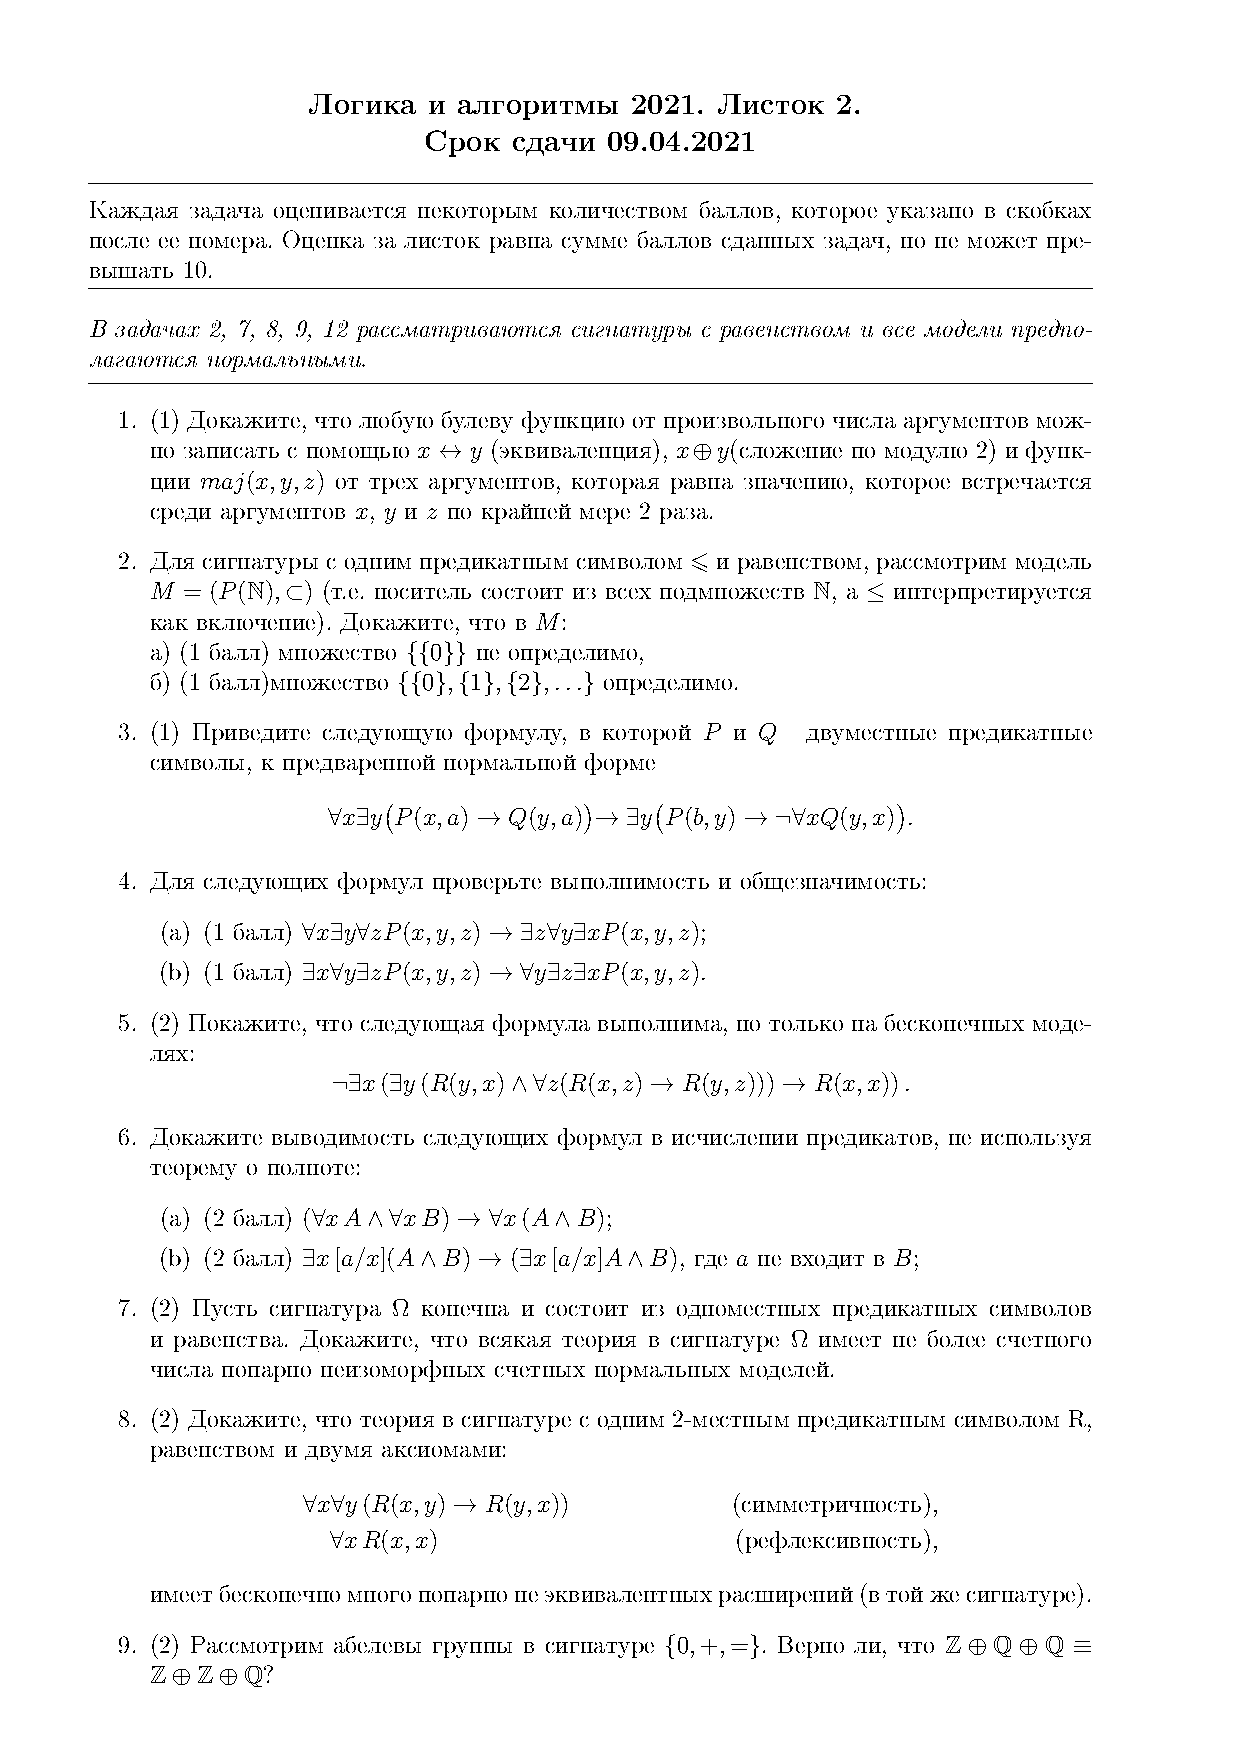
\includepdf[scale=1,pages=1-2]{Tasks/listok2}
\newpage
\section*{Решения}
\subsection*{Задача 1}
	Теорема о функциональной полноте. Для любой функции $\varphi: \mathbb{B}^n \to \mathbb{B}$ найдется такая формула $A$ от $n$ переменных, что $\varphi = \varphi_{A}$. При этом можно считать, что $A$ содержит лишь связки $\neg$ и $\vee$.\\
	Следовательно если выразить $\neg$ и $\vee$ через $x \leftrightarrow y,\ x \oplus y,\ \operatorname{maj}(x,y,z)$\\
	\begin{gather*}
	\begin{tabular}{ c c c c c c }
		x & y & x \leftrightarrow y & x \oplus y & \operatorname{maj}(x, y, x \oplus y) & x \oplus (x \leftrightarrow x)\\
		0 & 0 & 1 & 0 & 0 & 1\\
		0 & 1 & 0 & 1 & 1 & 1\\
		1 & 0 & 0 & 1 & 1 & 0\\
		1 & 1 & 1 & 0 & 1 & 0
	\end{tabular}
	\end{gather*}
	Заметим, что $\operatorname{maj}(x, y, x \oplus y)$ соответствует $x \vee y$, а $x \oplus (x \leftrightarrow x) = x \oplus 1$ соответствует $\neg x$, а следовательно любую булеву функцию можно записать, используя только данные по условию функции.

\subsection*{Задача 2}
\begin{enumerate}
\item[(a)] Рассмотрим отображение, такое что $\{0\} \leftrightarrow \{1\}$. Покажем, что это автоморфизм, то есть что если $A \subseteq B$, то $A' \subseteq B'$. Пусть $a \in A'$
	\begin{gather*}
		a \ne 0,1 \Rightarrow a \in A \Rightarrow a \in B \Rightarrow a \in B'\\
		a = 0 \Rightarrow 1 \in A \Rightarrow 1 \in B \Rightarrow 0 \in B'\\
		a = 1 \Rightarrow 0 \in A \Rightarrow 0 \in B \Rightarrow 1 \in B'
	\end{gather*}
	Итак, множество $\{\{0\}\}$ не сохранилось при рассмотренном автоморфизме, а определимые множество сохраняются при любом автоморфизме, а следовательно $\{\{0\}\}$ не явояется определимым.

\item[(b)]
	Зададим предикат, выражающий свойство одноэлементности множества, то есть всякое подмножество данного множества или пусто, или совпадает с ним самим. Выразим свойство пустоты множества ($x = \{\}$) формулой $\forall y\ x \leqslant y$, а также свойство равенства двух подмножеств ($x = y$) формулой $(x \leqslant y) \wedge (y \leqslant x)$. Через это мы можем выразить свойство одноэлементности $\forall y ((y \leqslant x) \to ((y = \{\}) \vee (y = x)))$.
\end{enumerate}
\vskip 0.4in

\subsection*{Задача 3}
	\begin{gather*}
		\forall x \exists y(P(x,a) \to Q(y,a)) \to \exists y(P(b,y) \to \neg \forall x Q(y,x))\\
		\forall x \exists y(P(x,a) \to Q(y,a)) \to \exists z(P(b,z) \to \neg \forall t Q(z,t))\\
		\forall x \exists y(\neg P(x,a) \vee Q(y,a)) \to \exists z(\neg P(b,z) \vee \neg \forall t Q(z,t))\\
		\neg \forall x \exists y(\neg P(x,a) \vee Q(y,a)) \vee \exists z(\neg P(b,z) \vee \neg \forall t Q(z,t))\\
		\neg \forall x \exists y(\neg P(x,a) \vee Q(y,a)) \vee \exists z(\neg P(b,z) \vee \exists t \neg Q(z,t))\\
		\exists x \forall y \neg (\neg P(x,a) \vee Q(y,a)) \vee \exists z(\neg P(b,z) \vee \exists t \neg Q(z,t))\\
		\exists x \forall y \exists z \exists t \neg (\neg P(x,a) \vee Q(y,a)) \vee (\neg P(b,z) \vee \neg Q(z,t))\\
		\exists x \forall y \exists z \exists t (P(x,a) \wedge \neg Q(y,a)) \vee (\neg P(b,z) \vee \neg Q(z,t))\\
		\exists x \forall y \exists z \exists t (P(x,a) \vee \neg P(b,z) \vee \neg Q(z,t)) \wedge (\neg Q(y,a) \vee \neg P(b,z) \vee \neg Q(z,t))\\
	\end{gather*}
\vskip 0.4in

\subsection*{Задача 4}
\begin{enumerate}
\item[(a)]
	\begin{gather*}
		\forall x \exists y \forall z P(x,y,z) \to \exists z \forall y \exists x P(x,y,z)
	\end{gather*}
	Рассмотрим модель целых чисел, в которой $P(x,y,z):\ y = x^2$. Тогда $\forall x \exists y \forall z (y = x^2)$ верно, а $\exists z \forall y \exists x (y = x^2)$ неверно, следовательно формула необщезначима.
\item[(b)]
	\begin{gather*}
		\exists x \forall y \exists z P(x,y,z) \to \forall y \exists z \exists x P(x,y,z)
	\end{gather*}
	Если левая часть -- истина, то существуют такие $x_0, z_0$, что $\forall y:\ P(x,y,z) \equiv 1$, тогда правая часть также истина, так как для этой же пары $x_0, z_0$ все будет выполнено, а следовательно формула истина. Если левая часть ложна, то следствие может быть любым, а следовательно формула также истина. Тогда она всегда истина, а следовательно выполнима и общезначима
\end{enumerate}
\vskip 0.4in

\subsection*{Задача 5}
	\begin{gather*}
		\neg \exists x(\exists y(R(y,x) \wedge \forall z(R(x,z) \to R(y,z))) \to R(x,x))\\
		\forall x \neg (\exists y(R(y,x) \wedge \forall z(R(x,z) \to R(y,z))) \to R(x,x))\\
		\forall x \neg (\exists y(R(y,x) \wedge \forall z(\neg R(x,z) \vee R(y,z))) \to R(x,x))\\
		\forall x \neg ( \neg \exists y(R(y,x) \wedge \forall z(\neg R(x,z) \vee R(y,z))) \vee R(x,x))\\
		\forall x (\exists y(R(y,x) \wedge \forall z(\neg R(x,z) \vee R(y,z))) \wedge \neg R(x,x))\\
		\forall x \neg R(x,x) \wedge \forall x \exists y (R(y,x) \wedge \forall z (\neg R(x,z) \vee R(y,z)))\\
		\forall x \neg R(x,x) \wedge \forall x \exists y \forall z (R(y,x) \wedge (\neg R(x,z) \vee R(y,z)))\\
		\forall x \exists y \forall z (\neg R(x,x) \wedge R(y,x) \wedge (\neg R(x,z) \vee R(y,z)))
	\end{gather*}

	\begin{comment}
		\forall x \neg R(x,x) \wedge \forall x \forall y \forall z (R(x,y) \wedge R(y,z) \to R(x,z)) \wedge \forall x\exists y R(x,y)\\
		\forall x \neg R(x,x) \wedge \forall x \forall y \forall z (\neg(R(x,y) \wedge R(y,z)) \vee R(x,z)) \wedge \forall x\exists y R(x,y)\\
		\forall x \neg R(x,x) \wedge \forall x \forall y \forall z (\neg R(x,y) \vee \neg R(y,z) \vee R(x,z)) \wedge \forall x\exists y R(x,y)
	Заметим что эта формула представляет из себя 2 аксиомы арифметики Пеано: $\forall x \exists y S(x) = y$ что то же самое что $\forall x \exists y R(x,y)$ и $\forall x \forall y S(x) = S(y) \to x = y$, что то же самое что $\forall x \forall y \forall z R(y,x) \wedge (\neg R(x,z) \vee R(y,z))$, этих аксиом достаточно для того, чтобы доказать бесконечность натуральных чисел, а следовательно данная форма выполнена только для бесконечных моделей
	\end{comment}
\vskip 0.4in

\subsection*{Задача 6}
\begin{enumerate}
\item[(a)]
	Правило Бернайса $\frac{A \to B}{A \to \forall x B[a/x]}$, следовательно нам достаточно доказать, что $(\forall x A \wedge \forall x B) \to A \wedge B$ выводимо.\\
	Применим теорему о дедукции: $\Gamma \vee \{P\} \vdash Q \Leftrightarrow \Gamma \vdash P \to Q$, то есть будем выводить $A \wedge B$ из аксиом и $(\forall x\ A \wedge \forall x\ B)$\\
	Аксиомы:\\
	$A \wedge B \to A$ (1), $A \wedge B \to B$ (2), $A \to (B \to A \wedge B)$ (3)\\
	$\forall x A[a/x] \to A[a/t]$ (4), $A[a/t] \to \exists x A[a/x]$ (5)\\
	Modus ponens: $\frac{A,\ A \to B}{B}$ (MP)
	\begin{gather*}
		\forall x A \wedge \forall x B \xrightarrow{\text{(1)}}
		\forall x A \xrightarrow{\text{(4)}}
		A \xrightarrow{\text{(*)}}
		A \wedge B
		\\
		\forall x A \wedge \forall x B \xrightarrow{\text{(2)}}
		\forall x B \xrightarrow{\text{(4)}}
		B\\
		\\
		\text{(*): } (A \to (B \to A \wedge B)) \xrightarrow{\text{(MP)}}
		(A \to A \wedge B) \xrightarrow{\text{(MP)}}
		A \wedge B
	\end{gather*}
\begin{comment}
\item[(b)]
	Правило Бернсайса: $\frac{B \to A}{\exists x\ B[a/x] \to A}$, следовательно достаточно доказать, что $A \wedge B \to \exists x [a/x]A \wedge B$ выводимо.\\
	Аналогично по теореме о дедукции выведем $\exists x [a/x] A \wedge B$ из аксиом $A \wedge B$
	\begin{gather*}
		A \wedge B\\
		A \text{ -- (1)}\\
		\exists x [a/x] A \text{ -- (5)}\\
		(B \to \exists x [a/x] A \wedge B) \text{ -- (3)}\\
		\exists x [a/x] A \text{ -- (MP)}\\
		\exists x [a/x] A \wedge B \text{ -- (MP)}
	\end{gather*}
	(в (3) в качестве $A$ выступает $\exists x [a/x] A$, в качестве $B -- B$)
	и
	\begin{gather*}
		A \wedge B\\
		B \text{ -- (2)}
	\end{gather*}
\end{comment}	
\end{enumerate}
\vskip 0.4in

\subsection*{Задача 9}
	Рассмотрим формулу
	\begin{gather*}
		\forall x (\forall s\ x \ne s + s) \to (\forall y (\forall t\ y \ne t + t) \to \exists w\ x + y = w + w)
	\end{gather*}
	Пусть $\mathbb{Z} \oplus \mathbb{Q} \oplus \mathbb{Q} = M_1,\ \mathbb{Z} \oplus \mathbb{Z} \oplus \mathbb{Q} = M_2$
	\vskip 0.1in
	Эта формула всегда верна в $M_1$:\\
	Пусть $x \ne s + s\ \forall s$, это значит, что $x = (\text{нечетное}, \text{любое}, \text{любое})$, так как га второй и третьей позиции рациональные числа, там можно любое число представить в виде $\frac{\text{число}}{2}$. Пусть $y \ne t+t$, тогда аналог $y = (\text{нечетное}, \text{любое}, \text{любое})$. Тогда $x + y = (\text{нечетное}, \text{любое}, \text{любое}) + (\text{нечетное}, \text{любое}, \text{любое}) = (\text{четное}, \text{любое}, \text{любое})$, то есть формула примет вид $1 \to (1 \to 1) = 1$\\
	Если $x \ne s + s,\ y = t + t$, то $x + y = (\text{нечетное}, \text{любое}, \text{любое})$ и формула примет вид $1 \to (0 \to 0) = 1 \to 1 = 1$\\
	Если $x = s + s,\ y \ne t + t$, то $x + y = (\text{нечетное}, \text{любое}, \text{любое})$ и формула примет вид $0 \to (1 \to 0) = 0 \to 0 = 1$\\
	Если $x = s + s,\ y = t + t$, то $x + y = (\text{четное}, \text{любое}, \text{любое})$ и формула примет вид $0 \to (0 \to 1) = 0 \to 1 = 1$
	\vskip 0.1in
	Но в $M_2$ эта формула не всегда верна, рассмотрим следующий случай:\\
	$x = (1,0,0),\ y = (0,1,0),\ x + y = (1,1,0)$. Тогда формула примет вид $1 \to (1 \to 0) = 1 \to 0 = 0$, то есть они не изоморфны и утверждение задачи неверно.

\end{document}